% ****** Start of file apssamp.tex ******
%
%   This file is part of the APS files in the REVTeX 4.2 distribution.
%   Version 4.2a of REVTeX, December 2014
%
%   Copyright (c) 2014 The American Physical Society.
%
%   See the REVTeX 4 README file for restrictions and more information.
%
% TeX'ing this file requires that you have AMS-LaTeX 2.0 installed
% as well as the rest of the prerequisites for REVTeX 4.2
%
% See the REVTeX 4 README file
% It also requires running BibTeX. The commands are as follows:
%
%  1)  latex apssamp.tex
%  2)  bibtex apssamp
%  3)  latex apssamp.tex
%  4)  latex apssamp.tex
%
\documentclass[%
 reprint,
%superscriptaddress,
%groupedaddress,
%unsortedaddress,
%runinaddress,
%frontmatterverbose, 
%preprint,
%preprintnumbers,
%nofootinbib,
%nobibnotes,
%bibnotes,
 amsmath,amssymb,
 aps,
%pra,
%prb,
%rmp,
%prstab,
%prstper,
%floatfix,
]{revtex4-2}

\usepackage{graphicx}% Include figure files
\usepackage{dcolumn}% Align table columns on decimal point
\usepackage{bm}% bold math
\usepackage{float}
\usepackage{epigraph} 


%\usepackage{hyperref}% add hypertext capabilities
%\usepackage[mathlines]{lineno}% Enable numbering of text and display math
%\linenumbers\relax % Commence numbering lines

%\usepackage[showframe,%Uncomment any one of the following lines to test 
%%scale=0.7, marginratio={1:1, 2:3}, ignoreall,% default settings
%%text={7in,10in},centering,
%%margin=1.5in,
%%total={6.5in,8.75in}, top=1.2in, left=0.9in, includefoot,
%%height=10in,a5paper,hmargin={3cm,0.8in},
%]{geometry}

\begin{document}


\title{What is intelligence? \\
\footnotesize Computational Neuroscience Course homework 01}% Force line breaks with \\

\author{Vahid Shamsaddini}
 \email{shamsvahid2@gmail.com}
% \affiliation{%
%  Authors' institution and/or address\\
%  This line break forced with \textbackslash\textbackslash
% }%



\date{\today}% It is always \today, today,
             %  but any date may be explicitly specified




%\keywords{Suggested keywords}%Use showkeys class option if keyword
                              %display desired
\maketitle

%\tableofcontents

% \section{\label{sec:level1} jh}
\paragraph{\large Moore's law:}
\textbf{Moore's Law} observes the doubling of transistors on microchips approximately every two years ($18$ months), leading to exponential growth in computing power. While the computing power of the \textbf{human brain} is increasing linearly at a very low rate. This makes it possible for computers to first reach the computing power of a single human brain and then the combined power of all human brains, a milestone scientists call the \textbf{singularity}, expected to occur by \textbf{2045}.
\begin{figure}[H]
    \centering
    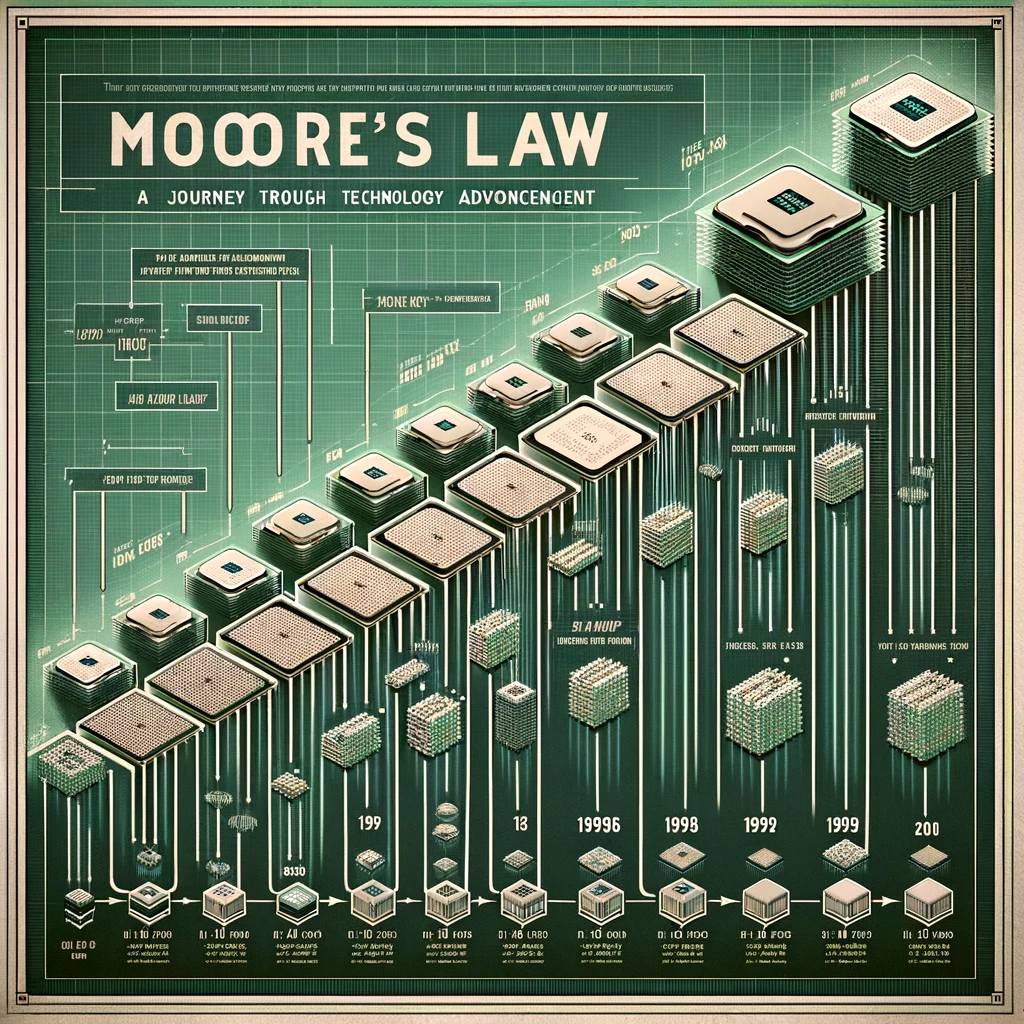
\includegraphics[width=0.25\textwidth]{images/gpt4_moore.png}
    \caption{\label{moore_law} A picture generated by GPT4 explaining Moore's law. I would suggest do not rely on numbers!}
\end{figure}
So, will they eliminate us all by 2045? Don't worry! This refers to computing power, not intelligence. Unlike us, computers require formal definitions and algorithms.
\begin{figure}[H]
    \centering
    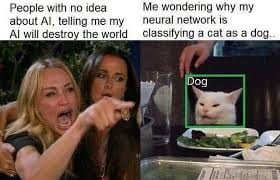
\includegraphics[width=0.350\textwidth]{images/silly_ai.jpeg}
    \caption{\label{silly_ai} No caption!!}
\end{figure}

\paragraph{\large What is intelligence?}
What is intelligence? We do not have an exact definition. However, we have some common understanding; for instance, an intelligent being will think, feel emotions, be conscious, and so on. Intelligence is a descriptive term that needs to be explained from your point of view.
\epigraph{I propose to consider the question, \textit{Can machines think?} This should begin with definitions of the meaning of the terms \textit{machine} and \textit{think}.}{\textit{ Turing 1950}}

\paragraph{\large Then what should we do?}
We need to understand the model of the brain to some extent and attempt to mimic it in the field of AI.
\begin{figure}[H]
    \centering
    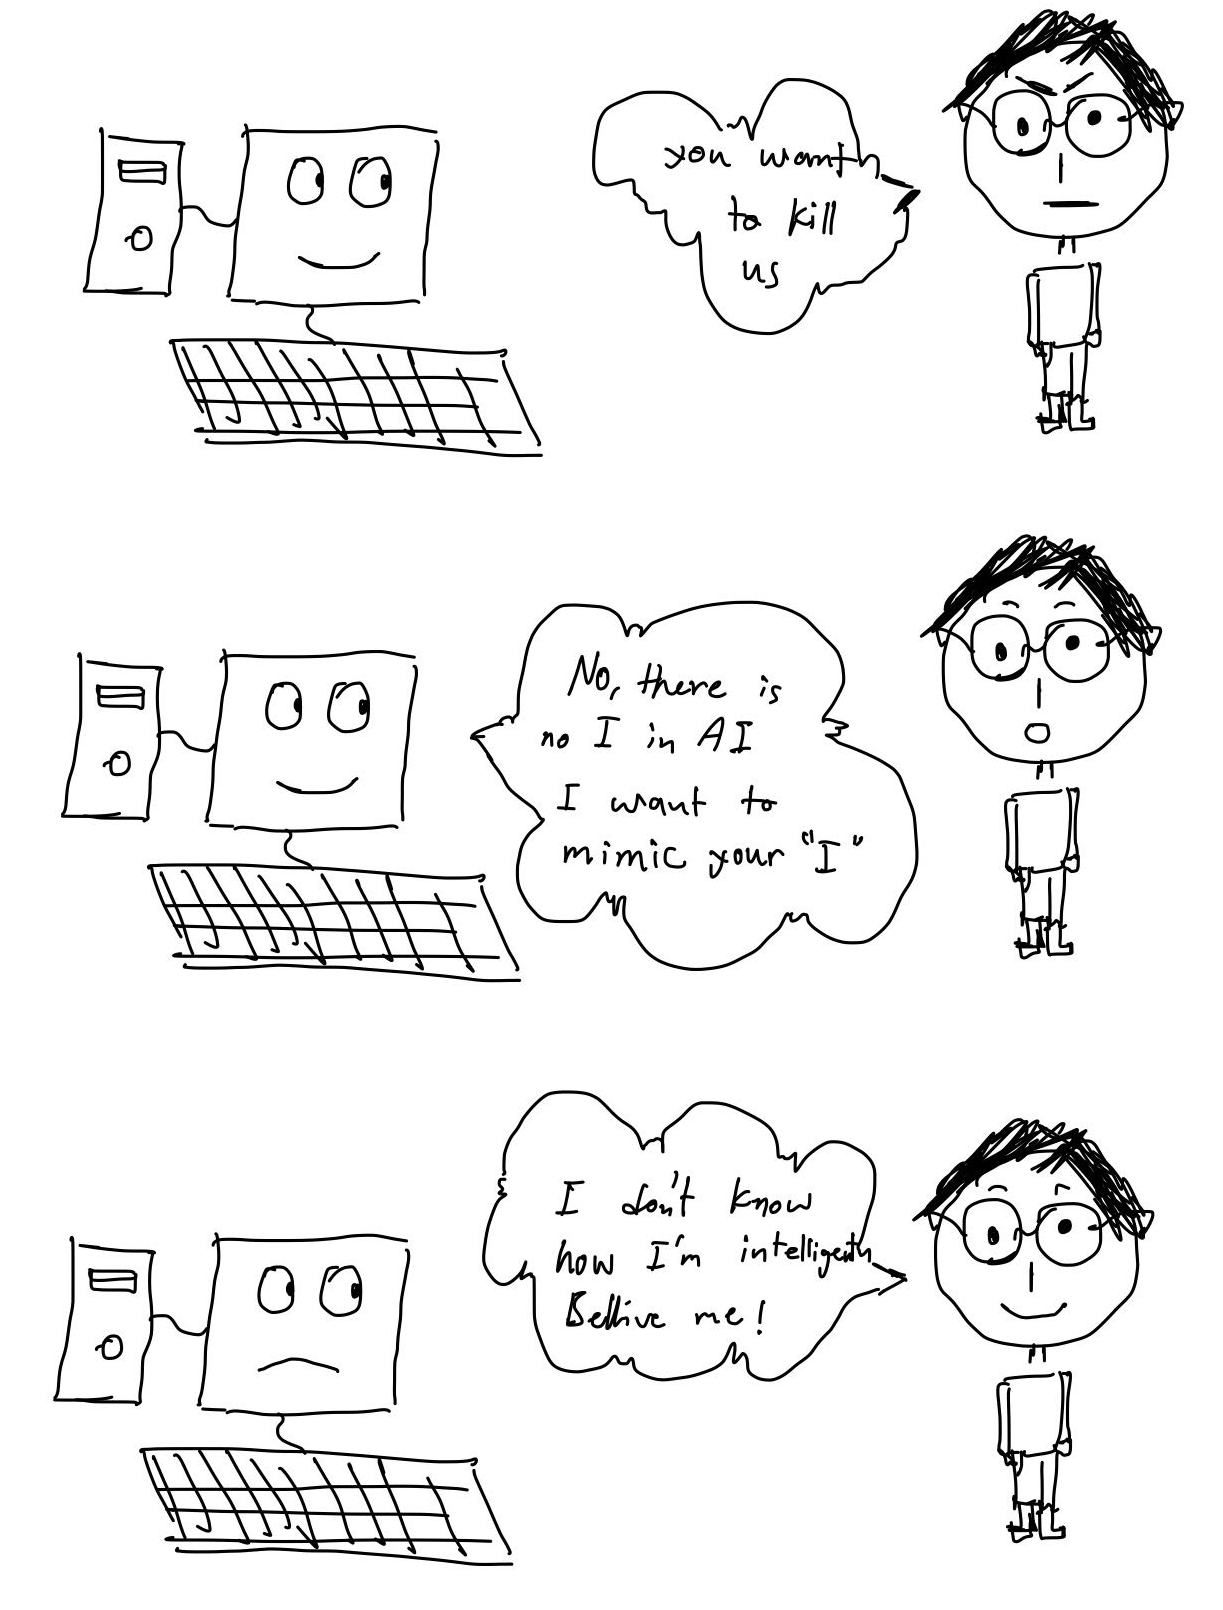
\includegraphics[width=0.5\textwidth]{images/mimic_human.png}
    \caption{\label{mimic_human_ai} AI-Neuroscience story! }
\end{figure}

\end{document}
%
% ****** End of file apssamp.tex ******
